\section{Realization}
\subsection{Experimental Setups}
%Bilder
The permanent magnetic field is provided by a large electromagnet connected to a power supply. The modulation of the magnetic field is created by two coils on the left and the right side of the sample holder. Those are connected to a sine voltage firstly and an adder at the end. There's an electromagnetic oscillating circuit between the respective ends of the iron cores of the electromagnet. There is a hole in the middle of it where the Hall sensor or the samples can be introduced. It's also connected to a frequency generator. An oscilloscope is connected to the modulating voltage to show its course just as to the oscillating circuit to show resonances.
\subsection{Experimental Approach}
Firstly, the homogeneity of the magnetic field inside the sample holder had to be proven using a Hall sensor. With this measurement, a working point was determined. The setup was the following:\\
\begin{figure}[htbp]
\begin{center}
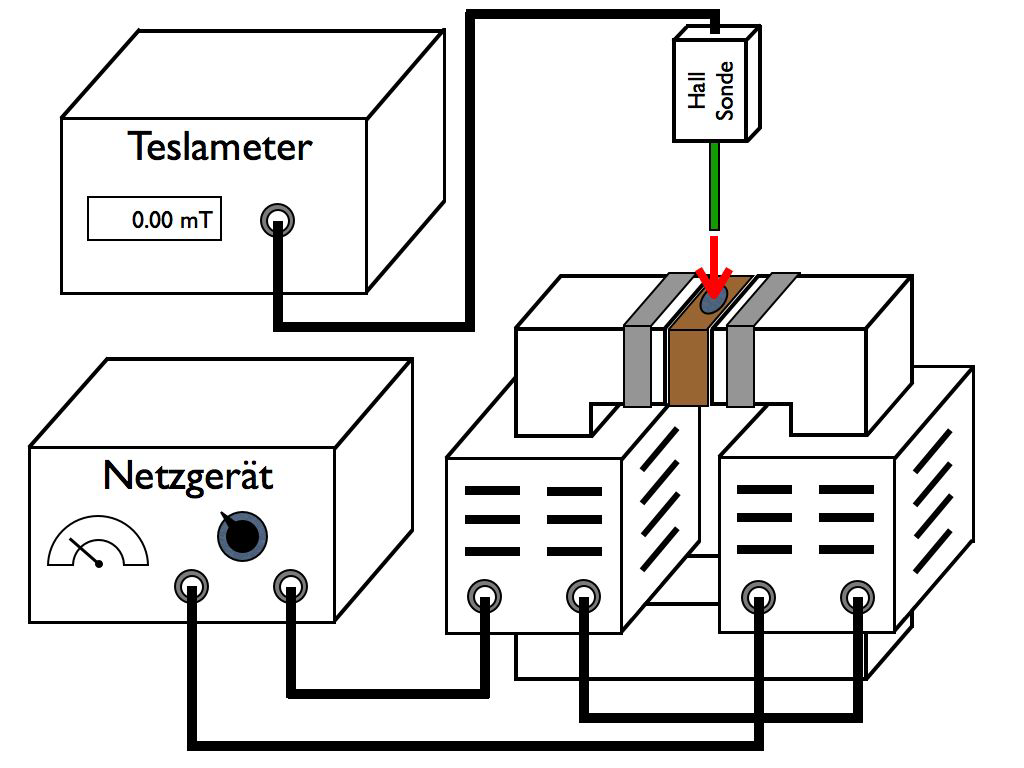
\includegraphics [scale=0.5]{Bilder/hallsonde.png}
\caption{Experimental setup for the determination of the homogeneity of the magnetic field (source: [ver])}
\end{center}
\end{figure}
\clearpage
Afterwards, hydrogen, glycol and Teflon samples were put inside the field one after the other with the intention to find their resonance frequency. A sine modulation was used to facilitate the realization of this part of the experiment: The resonance is passed by twice per sine period. Thus in the resulting absorption curve, one gets two absorption minima. To find the resonance frequency, the minima need to be equidistant, because that way they are at the zero of the modulation, which is at the appointed frequency of the radiation field. The setup and the expected curves can be seen below:\\
\begin{figure}[htbp]
\begin{center}
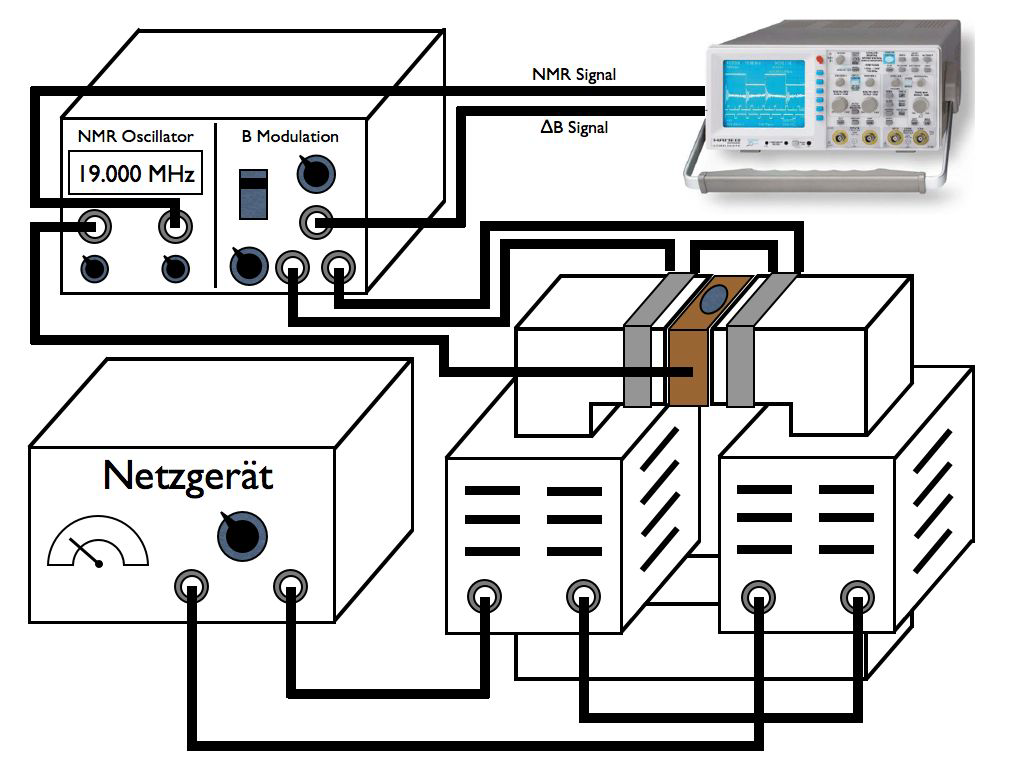
\includegraphics [scale=0.5]{Bilder/teil234.png}
\caption{Experimental setup for the determination of the resonance frequency with the sine-modulation (source: [ver])}
\end{center}
\end{figure}
\begin{figure}[htbp]
\begin{center}
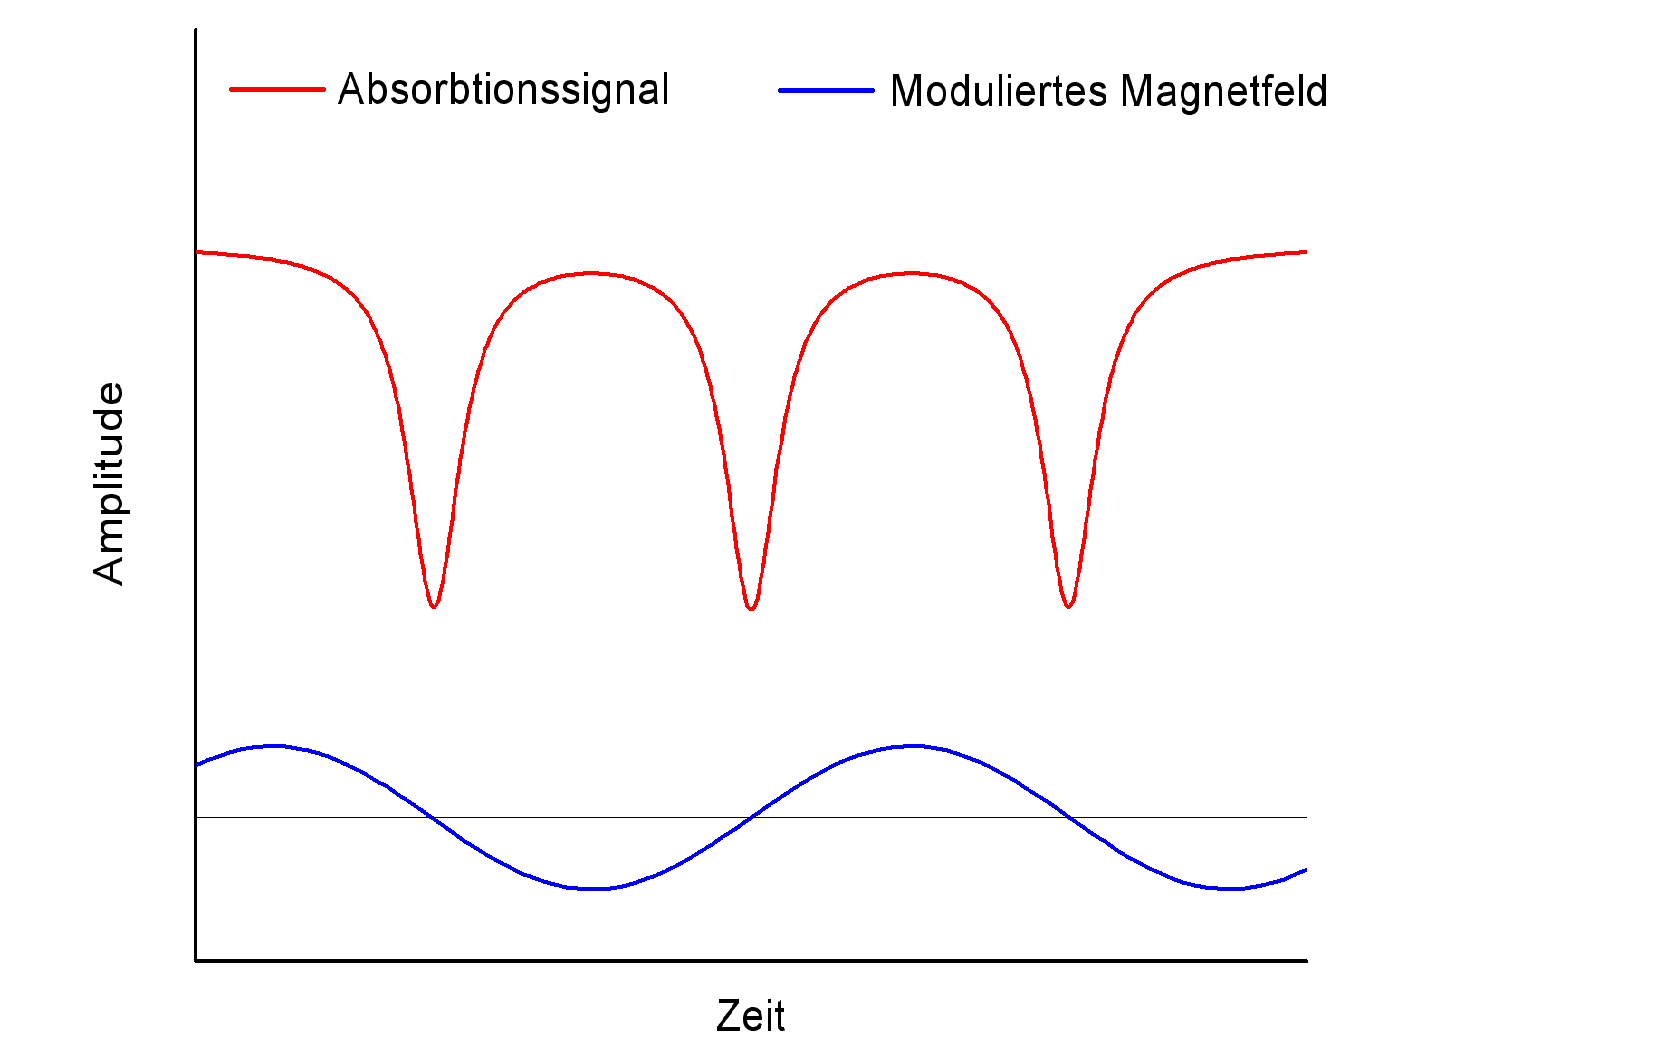
\includegraphics [scale=0.5]{Bilder/theoverlauf1.png}
\caption{Expected curves (source: [ver])}
\end{center}
\end{figure}
\clearpage
To get a better result for hydrogen, we use the lock-in method: a sawtooth voltage is applied as modulation, overlapped by a sine voltage with much lower amplitude and much higher frequency. The differences between the zero of the derived absorption curve and the sine-modulated sawrooth signal in time $\Delta t$ were measured for different frequencies. By using a linear fit, the resonance frequency could be determined (that's the frequency at $\Delta t=0s$). The setup and the expected curves look the following:\\
\begin{figure}[htbp]
\begin{center}
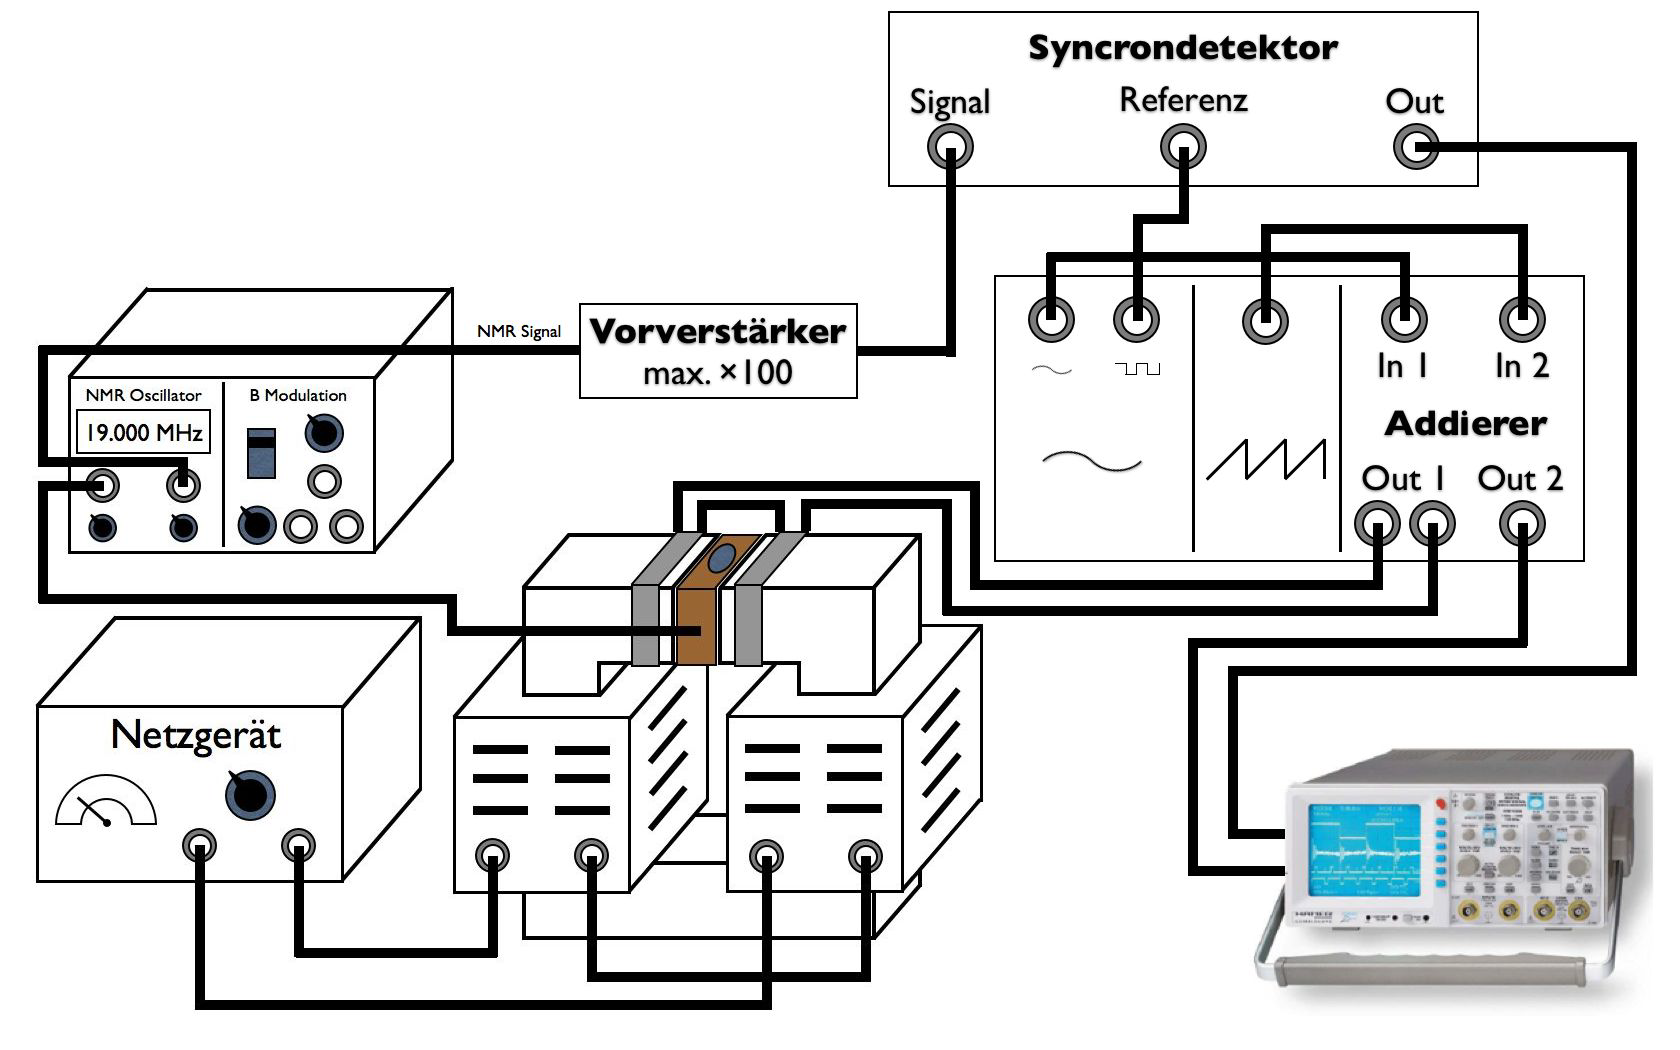
\includegraphics [scale=0.4]{Bilder/lockin.png}
\caption{Lock-in method (source: [ver])}
\end{center}
\end{figure}
\begin{figure}[htbp]
\begin{center}
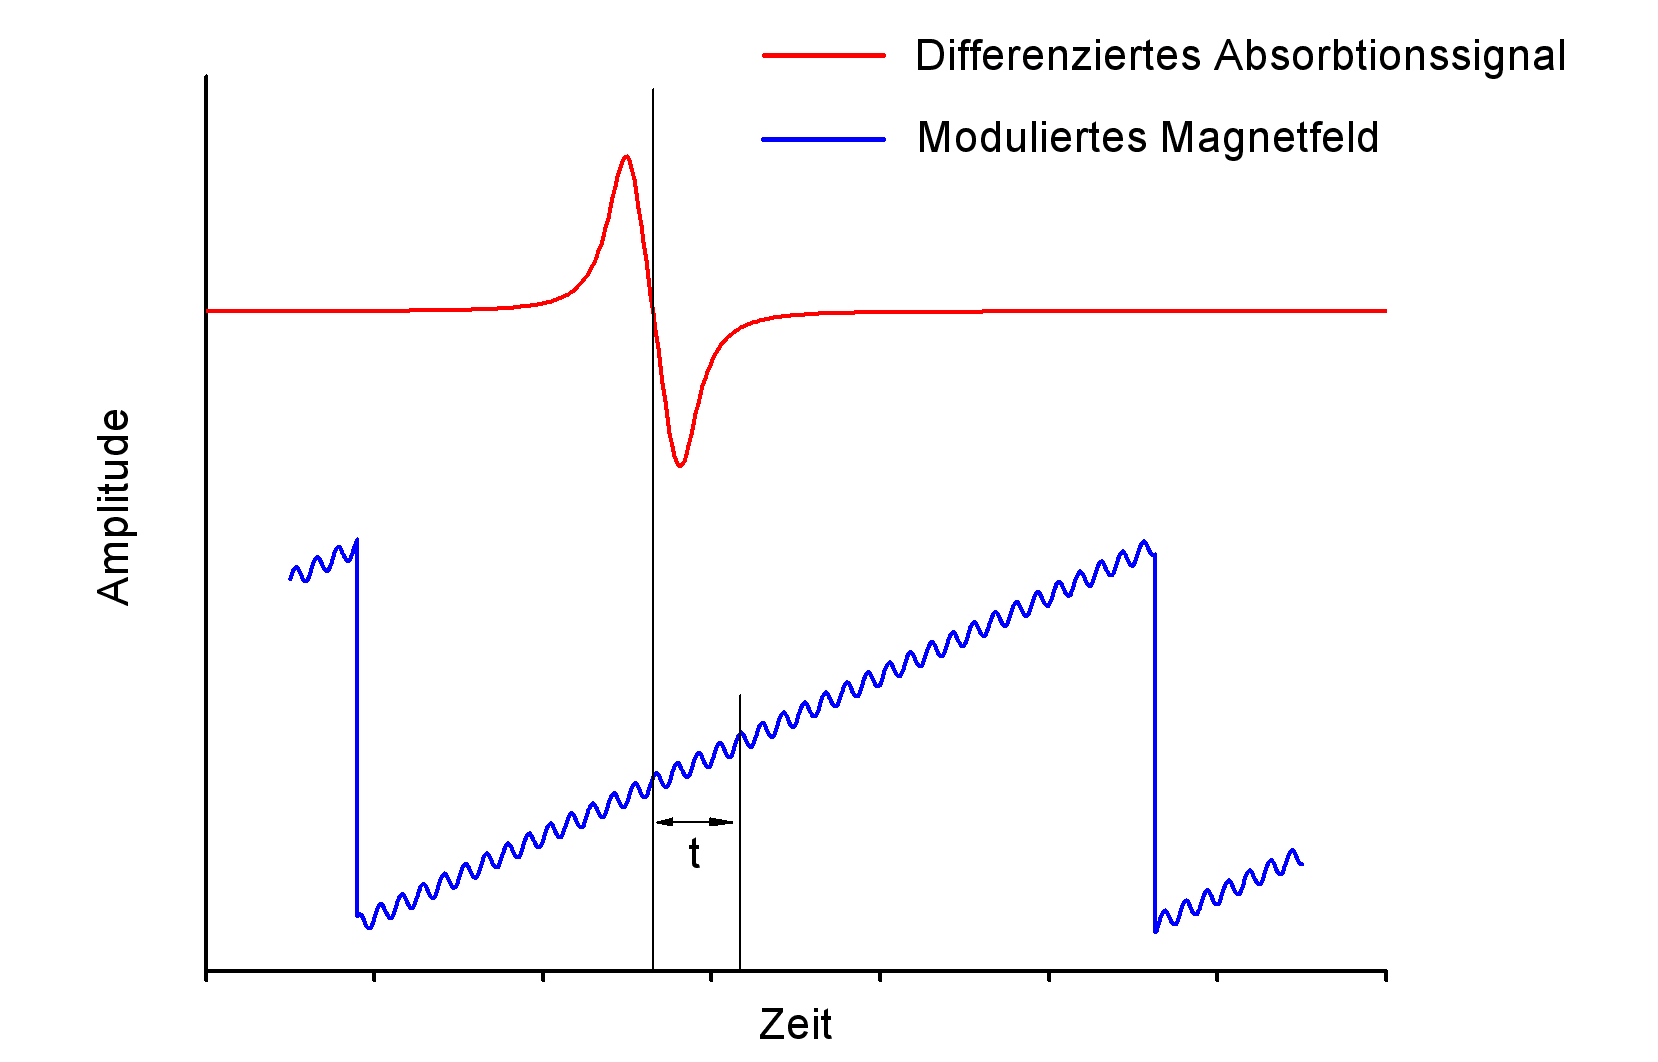
\includegraphics [scale=0.4]{Bilder/theoverlauf2.png}
\caption{Expected curves for the lock-in method (source: [ver])}
\end{center}
\end{figure}
\clearpage
